\section{Control Regions to validate backgrounds}\label{sec:control}

A set of different control regions is established to check that various background estimations are well modeled through the usage of the MC simulation and
data-driven methods. The regions are chosen to mimic the signal region topology as closely as possible, while remaining unaffected by the presence of new physics, so that they can be used to determine the accuracy of the background modeling without introducing any bias.

Two regions are defined:
\begin{itemize}
\item Photon + Jet control region defined by the loose selection criteria.
\item $W\gamma$ control region defined by the final state $W(\rightarrow l \nu)$ with the  charged lepton falling inside the detector acceptance;
\end{itemize}   

\label{sec:control}
\subsection{Photon + Jet Control Region}
To check the accuracy by which the backgrounds have modeled the data we look in regions dominated by backgrounds and with relatively little signal. One such region is dominated by $\gamma +$ jets when we do not cut on fake \met discriminators. The following cuts are imposed:

\begin{itemize}
\item \et$^{\gamma} > 45 \GeV $
\item $|\eta^{\gamma}| < 1.442$
\item $\sigma_{i{\eta}i{\eta}} > 0.001$ , $\sigma_{i{\phi}i{\phi}} > 0.001$ , swiss cross $> 0.9$ , $ 1.0 > R_{9} > 0.9$
\item \met$ > 40 $
\item Lepton Veto
\end{itemize}

Although our signal is present in this region, it is multiple orders of magnitude smaller than the expected background. The yields are shown in Table \ref{tab:pg_CR} and the photon \pt and \met distributions for this region are shown in Fig.~\ref{fig:pg_CR}.


\begin{figure}[!hp]
\centering
{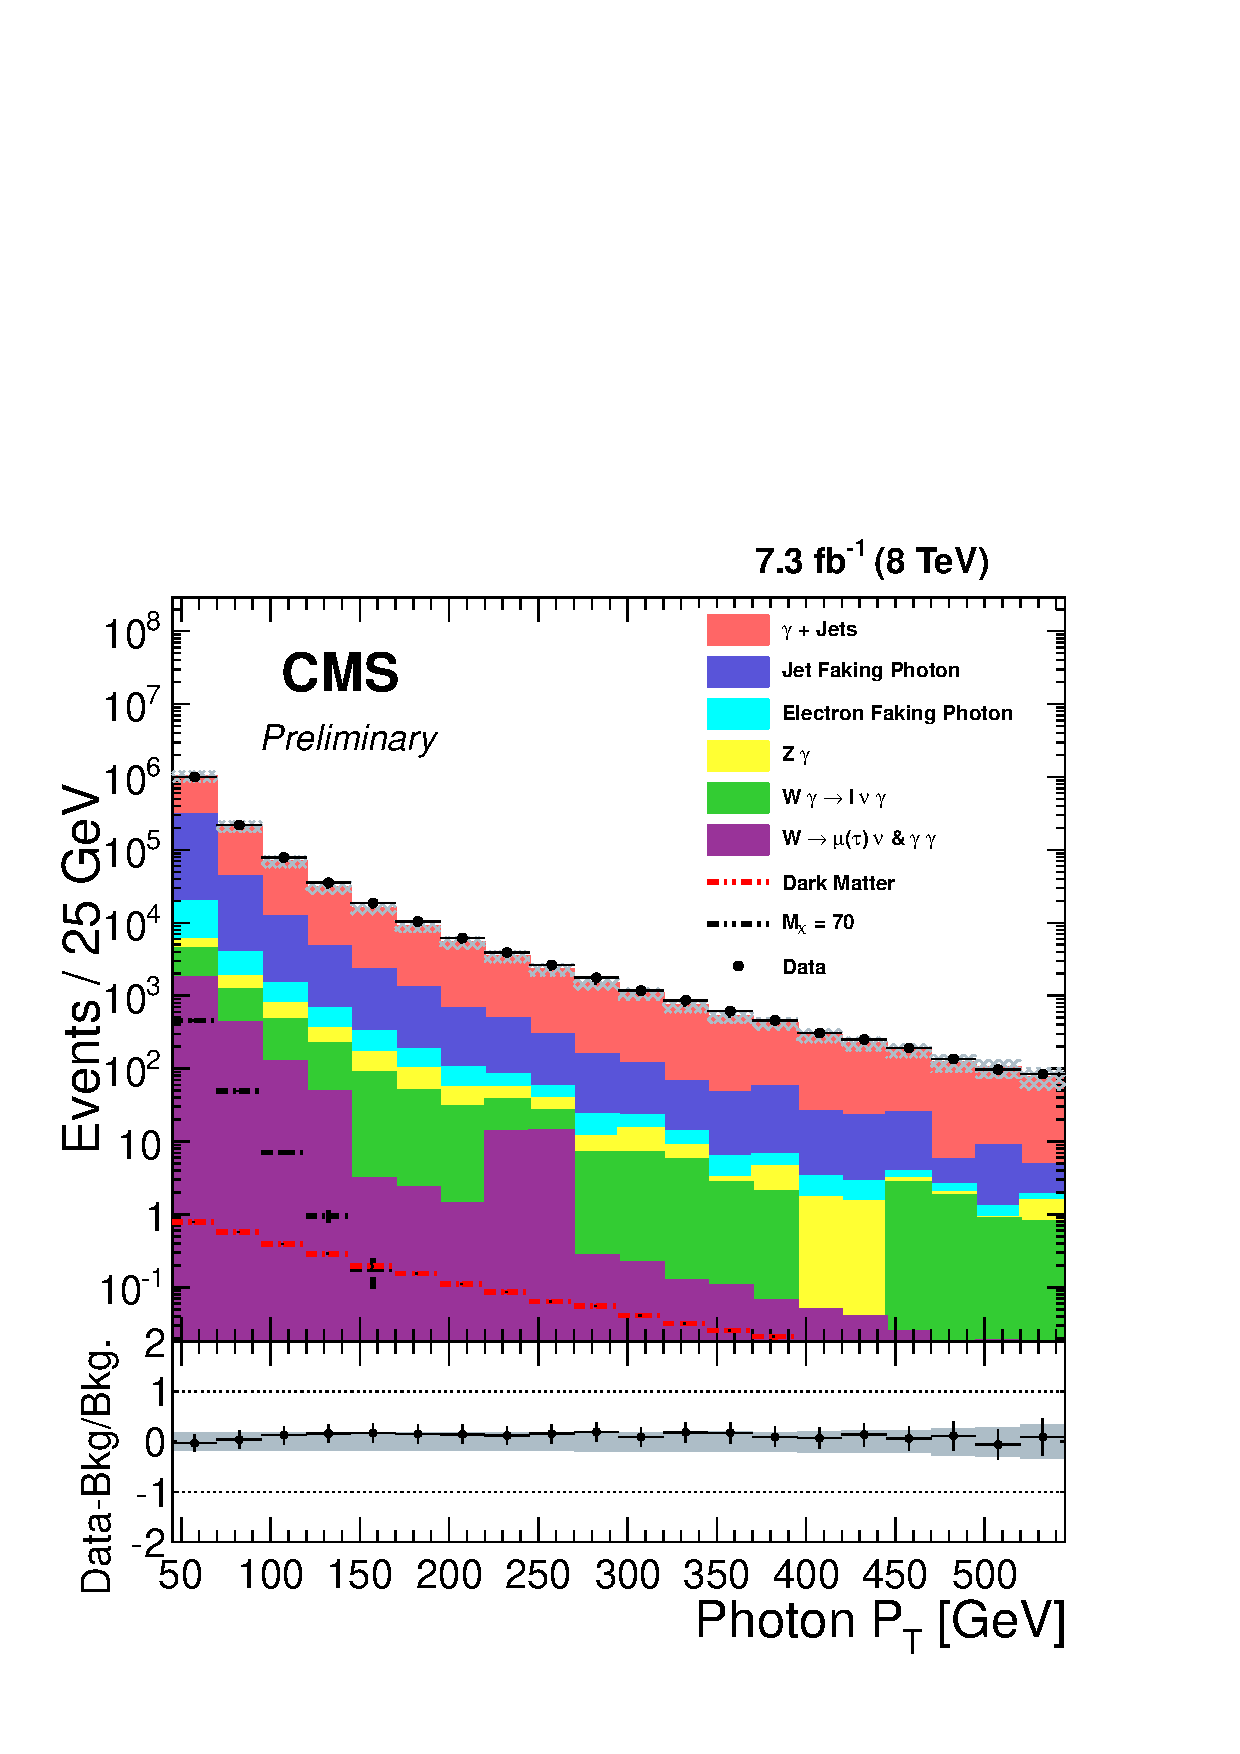
\includegraphics[scale=0.4]{analysis_figs/QCD_pt.pdf}}
{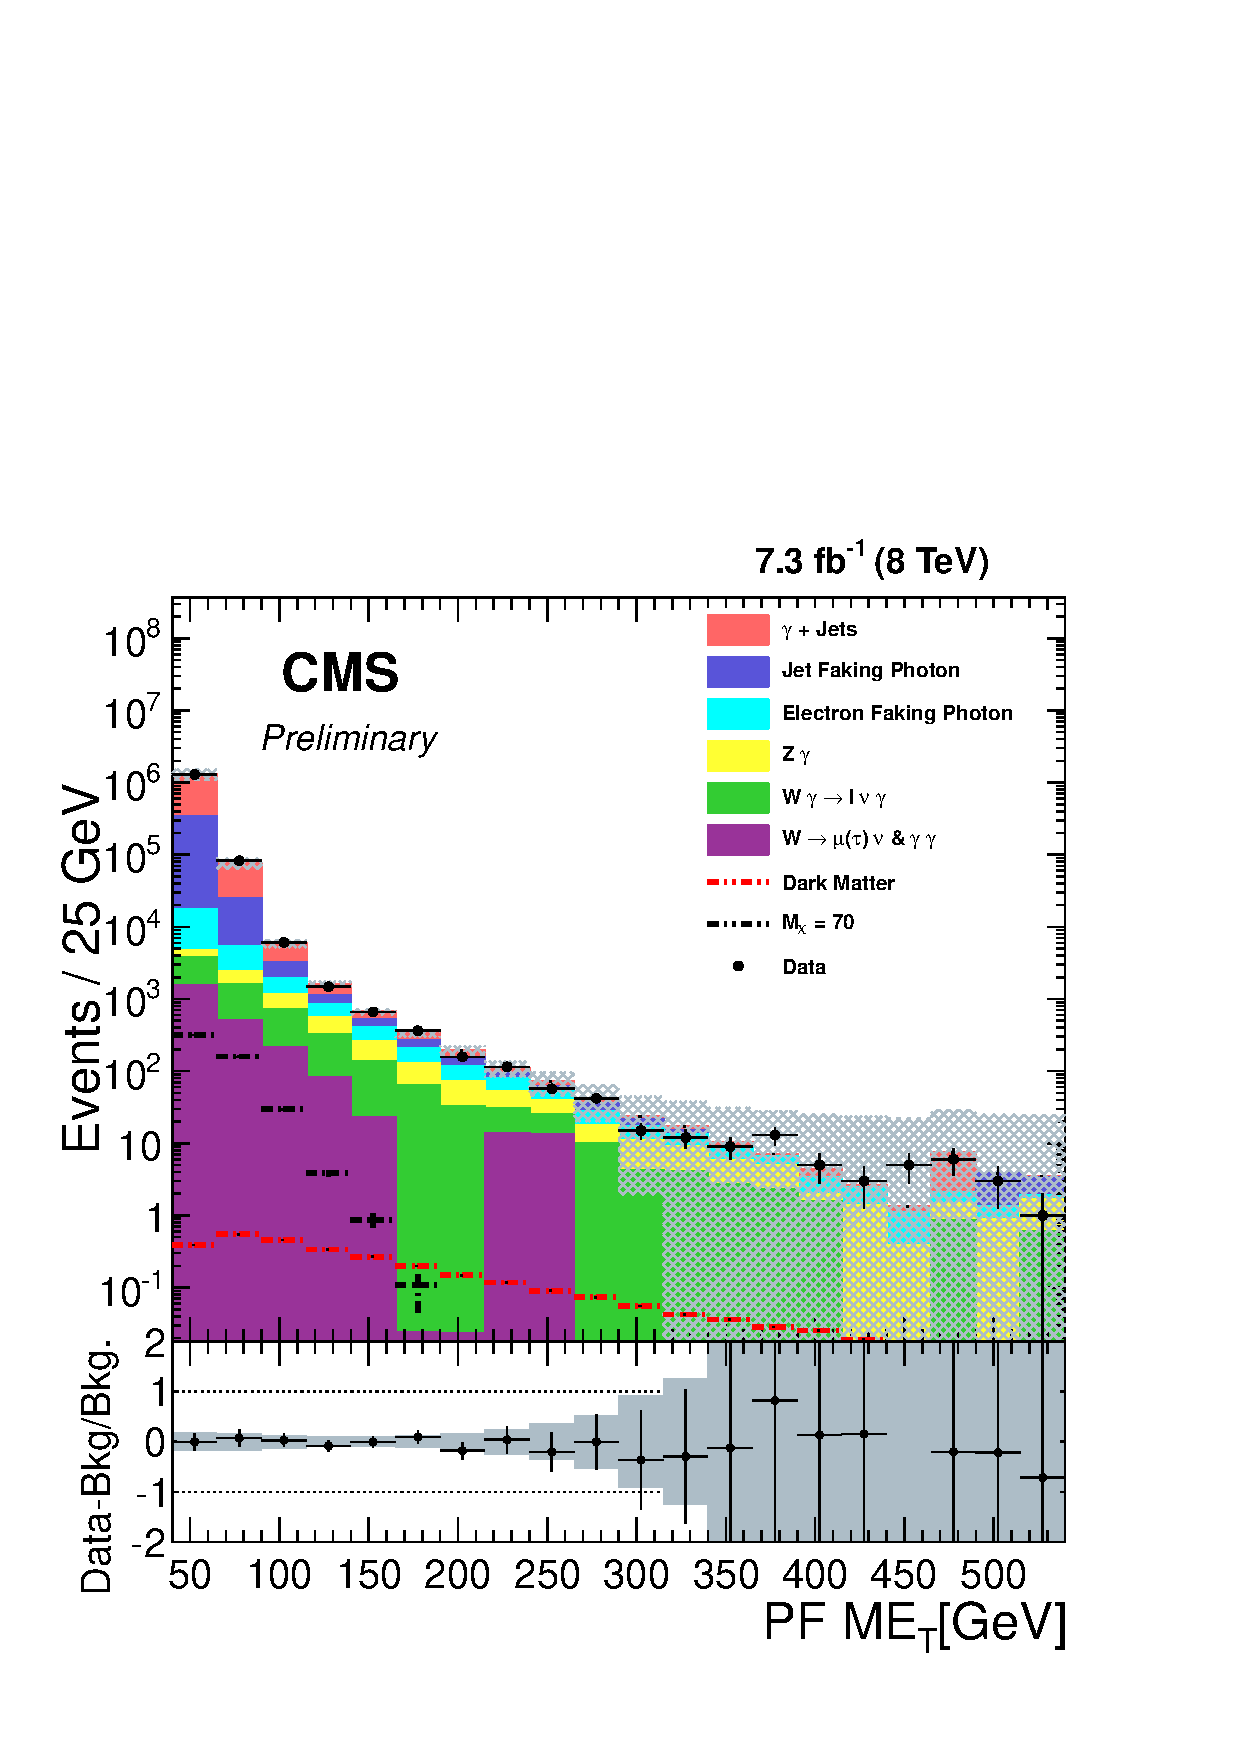
\includegraphics[scale=0.4]{analysis_figs/QCD_met.pdf}}
%\newline
\caption{Data vs background prediction comparison for the photon \pt and the \met in the $\gamma +$ jet control region.}
\label{fig:pg_CR}
\end{figure}

\begin{table}[!h]
\center
{
\begin{tabular}{|c|c|}
\hline
Process & Estimate \\
\hline
$\gamma +$ jets                          & $(1012 \pm 162 ) x 10^3$ \\
${\rm jet}\rightarrow \gamma$        & $(344 \pm 120 ) x 10^3$ \\
${\rm e} \rightarrow \gamma$         & $(171 \pm 10 ) x 10^2$ \\
$W(\to \ell\nu)+\gamma $                 &  $4242 \pm 212$ \\
$Z( \to \nu \bar{\nu} )+\gamma    $      &  $2457 \pm 122$ \\
Other                                    &  $27124 \pm 44$ \\
\hline
Total background                       &   $(1383 \pm 284 ) x 10^3$ \\
\hline
Data                                   &  $1386 x 10^3$  \\
\hline
\end{tabular}
\caption{Expected yields after the $\gamma +$ jets control region selections. Other backgrounds include $W\mu(\tau)\nu$, $Zll\gamma$ and $\gamma\gamma$.}
\label{tab:pg_CR}}
\end{table}

In this region background predictions and data are consistent within the uncertainty. However we realized due to possible mis-modeling of the $\gamma + $ jets background, the $\Delta \phi (\met,\gamma)$ distribution shows a shape discrepancy. To account for this discrepancy, we re-weighted the  $\gamma + $ jet background with respect to the data shape in this region. We subtracted all other backgrounds from data except $\gamma$ + jets and then applied the ratio of remaining data to  $\gamma + $ jets to the  $\gamma + $ jets background. Through this re-weighting, the modulation in the transverse mass distribution also disappears. Both  $\Delta \phi (\met,\gamma)$  and the transverse mass distributions can be seen in Fig. \ref{fig:pg_rw} and ~\ref{fig:MT}.

\begin{figure}[!hp]
\centering
{\label{fig:pg_rw_phi_b}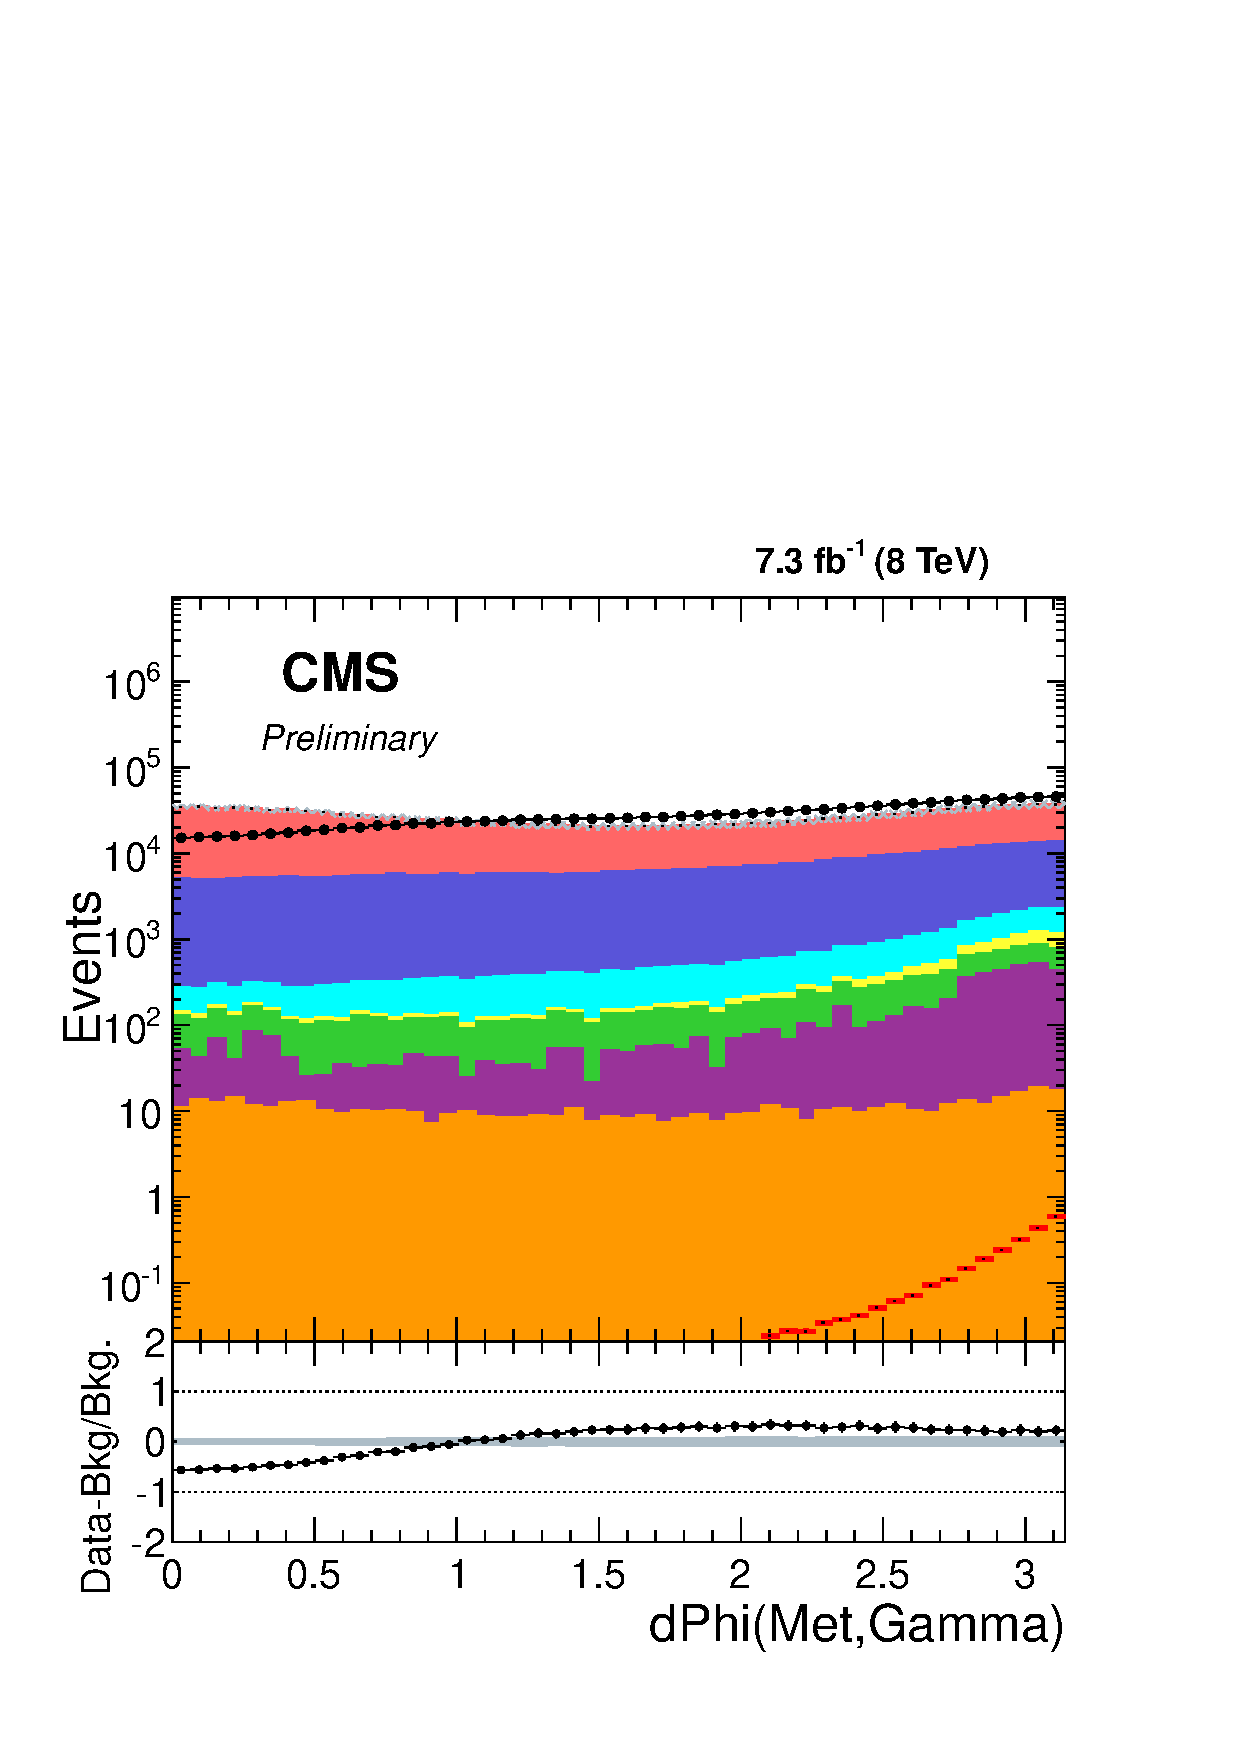
\includegraphics[scale=0.4]{analysis_figs/dphi_noreweight.pdf}}
{\label{fig:pg_rw_phi_a}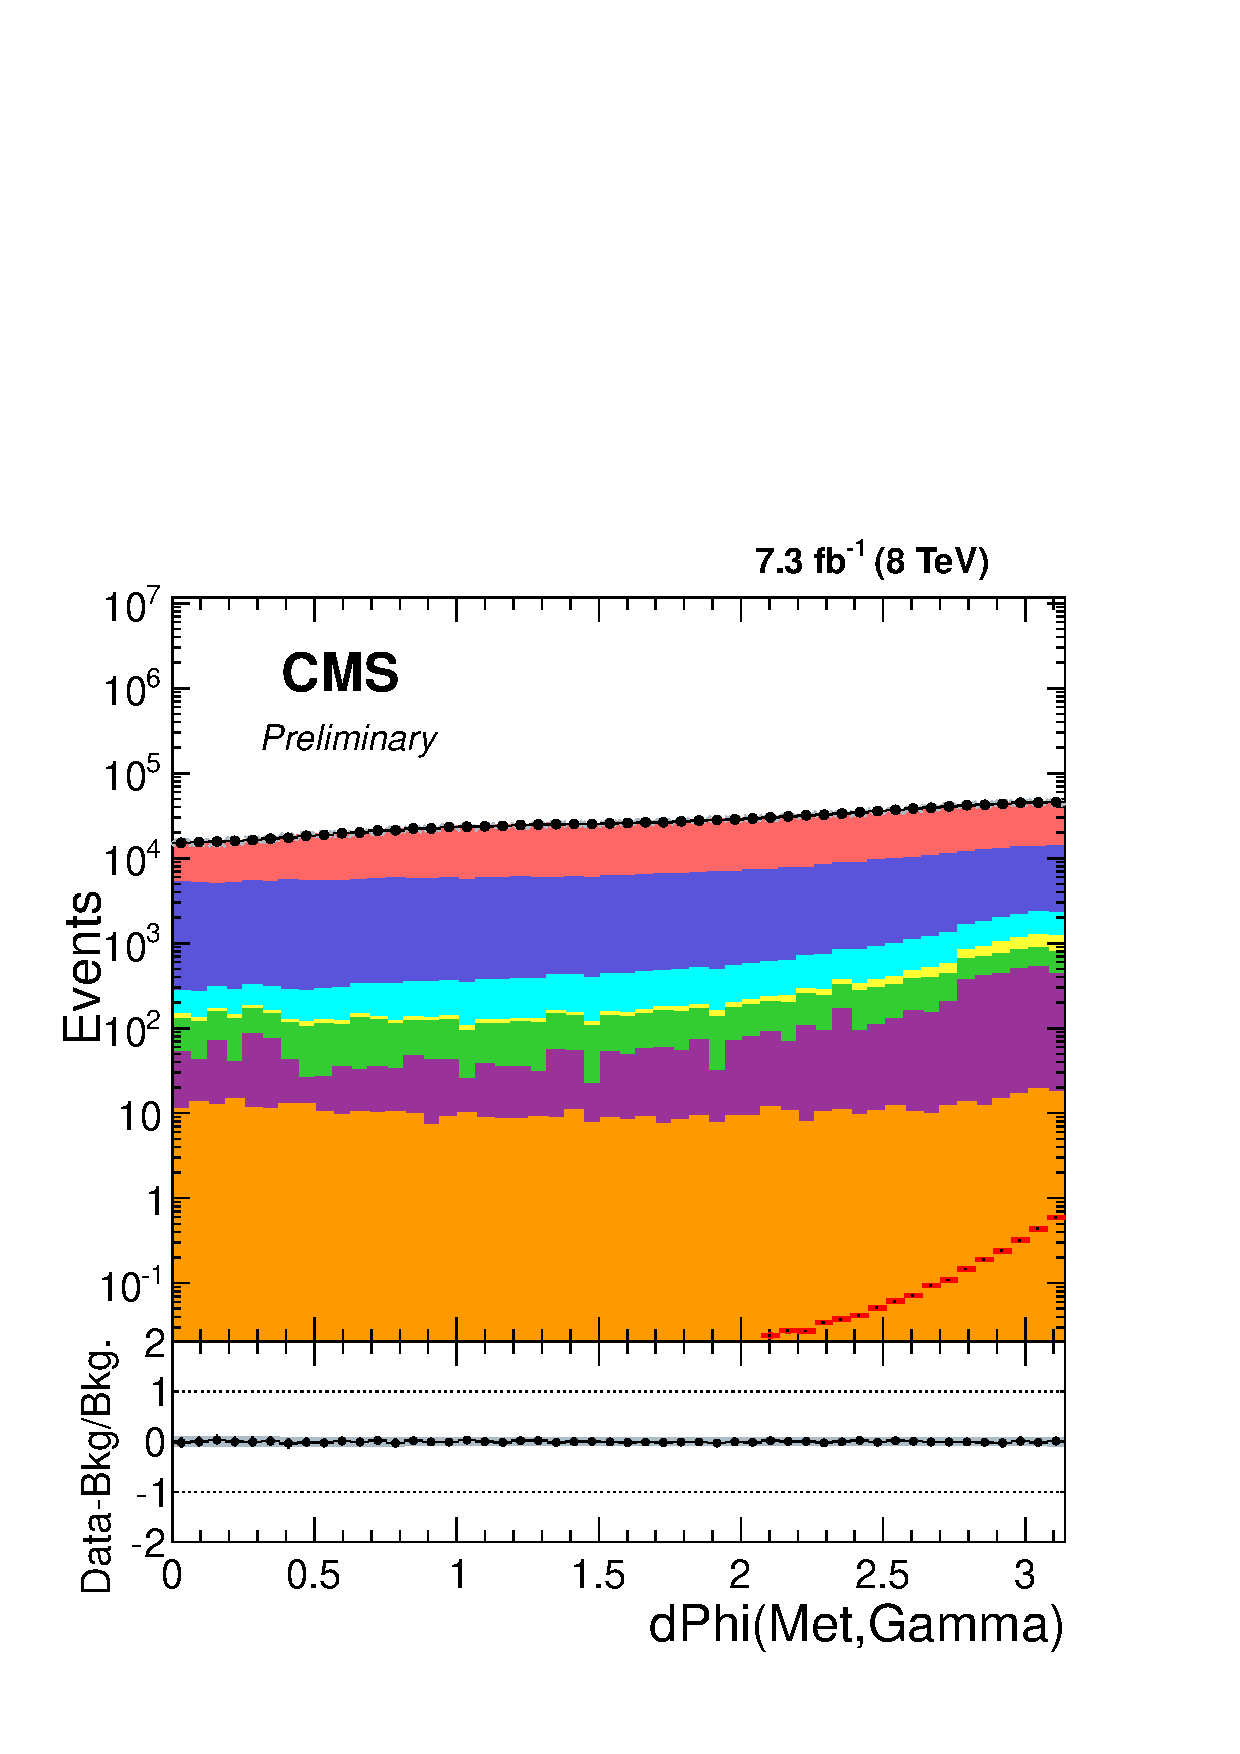
\includegraphics[scale=0.4]{analysis_figs/dphi_reweight.pdf}}
\caption{ Data vs background prediction comparison for the $\Delta \Phi (\gamma, \met)$ before and after the reweighting of the  $\gamma + $ jet background.}
\label{fig:pg_rw}
\end{figure}

\begin{figure}[!hp]
\centering
{\label{fig:mt_b}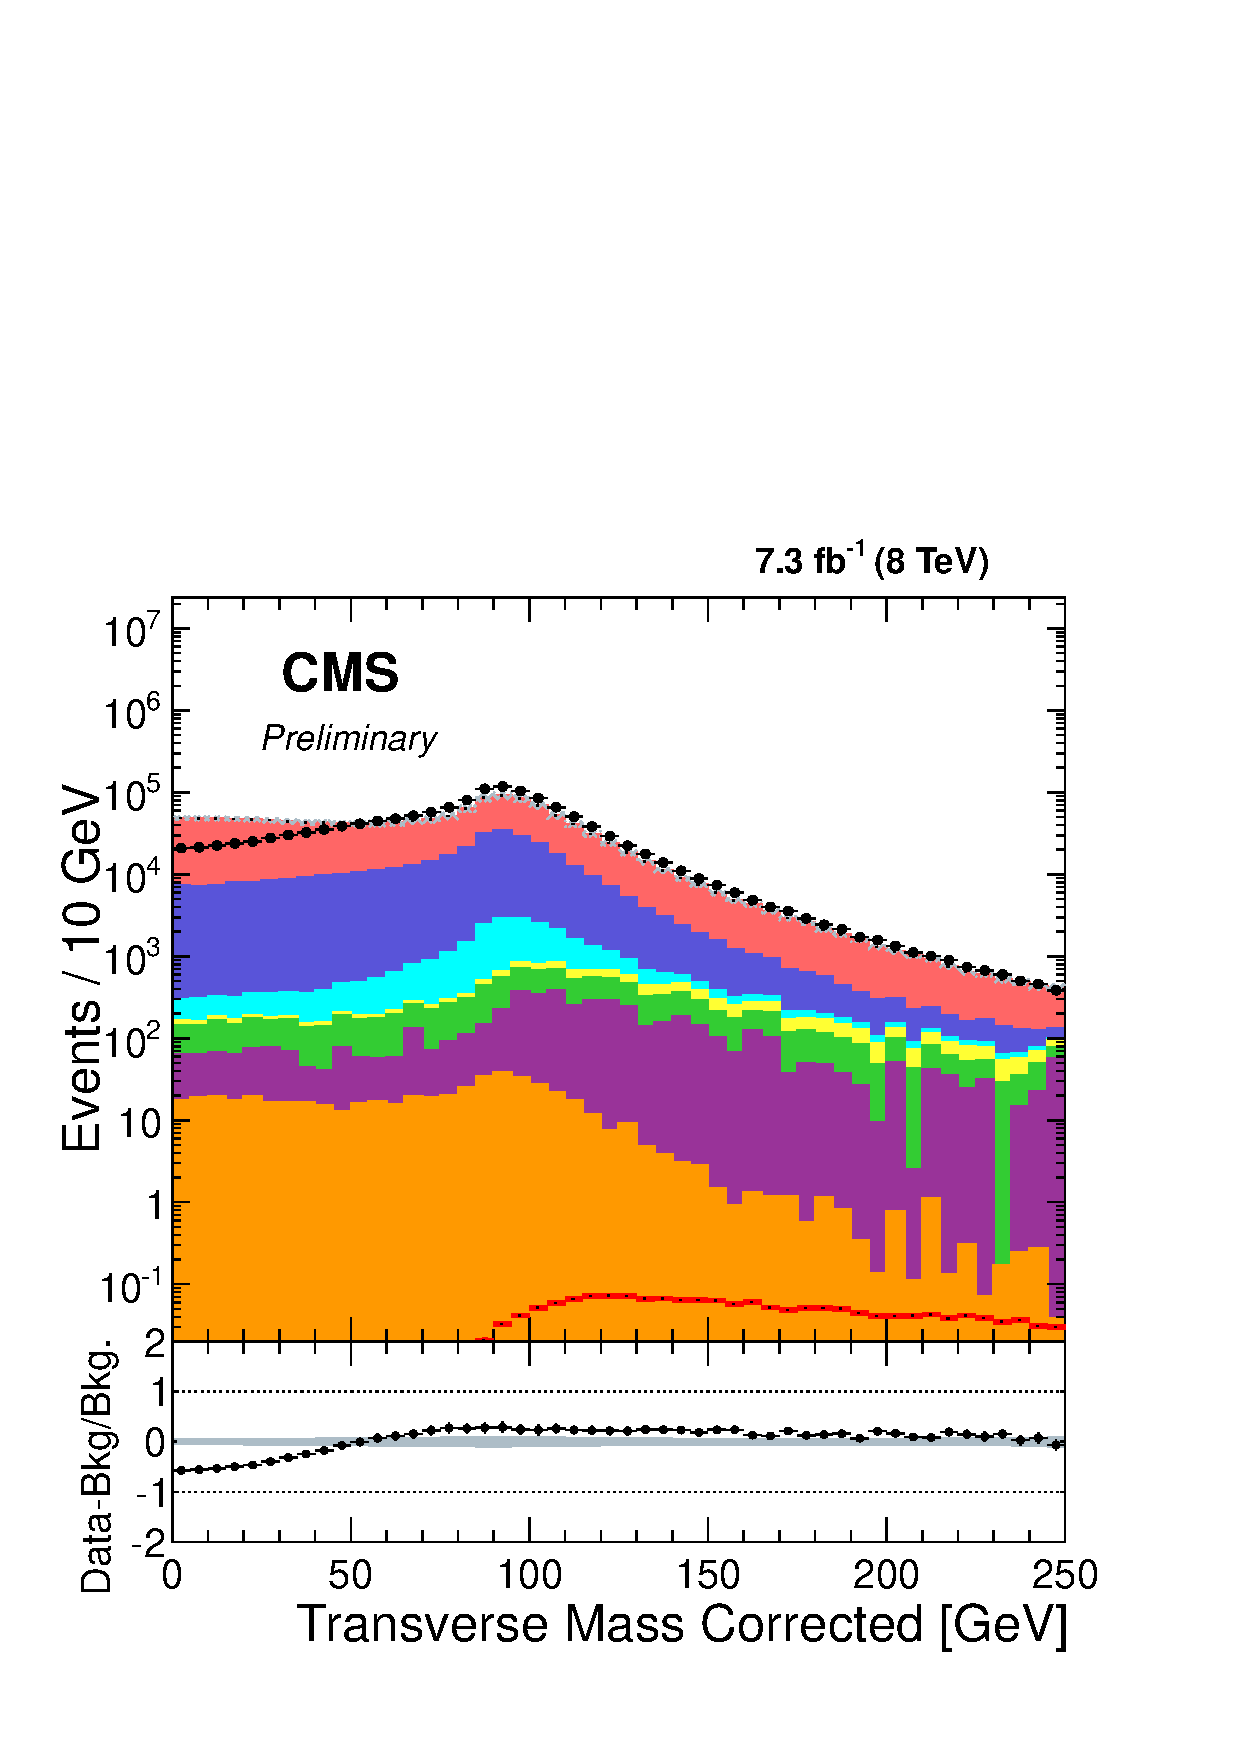
\includegraphics[scale=0.4]{analysis_figs/mt_b.pdf}}
{\label{fig:mt_a}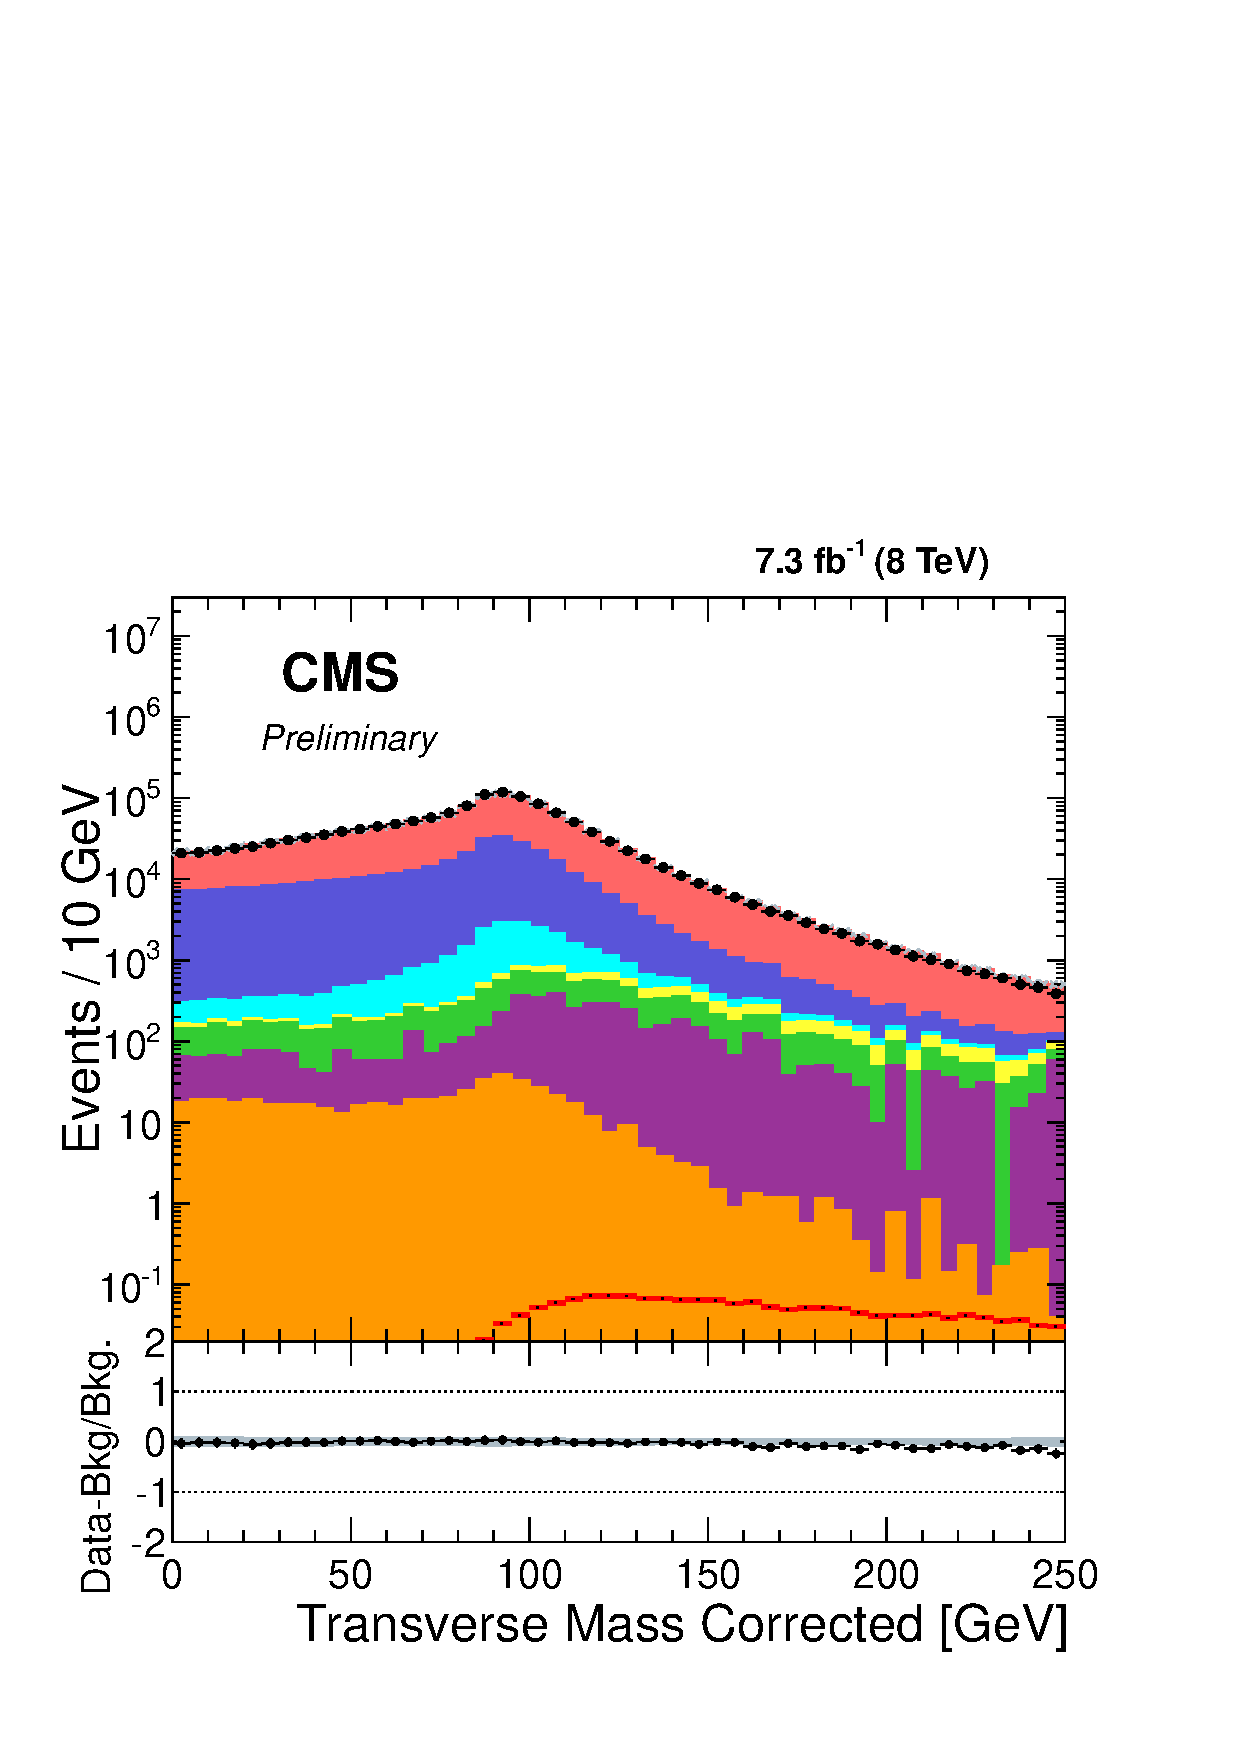
\includegraphics[scale=0.4]{analysis_figs/mt_a.pdf}}
\caption{ Data vs background prediction comparison for the MT distribution before and after the reweighting of the  $\gamma + $ jet background for $\Delta \Phi (\gamma, \met)$.}
\label{fig:MT}
\end{figure}

Lastly, we show the NJet and HT distributions for the pre-selection level after all the corrections that have been described in the text in Fig.~\ref{fig:control_jet}

\begin{figure}[!hp]
 \centering
  {\label{fig:njetfinal}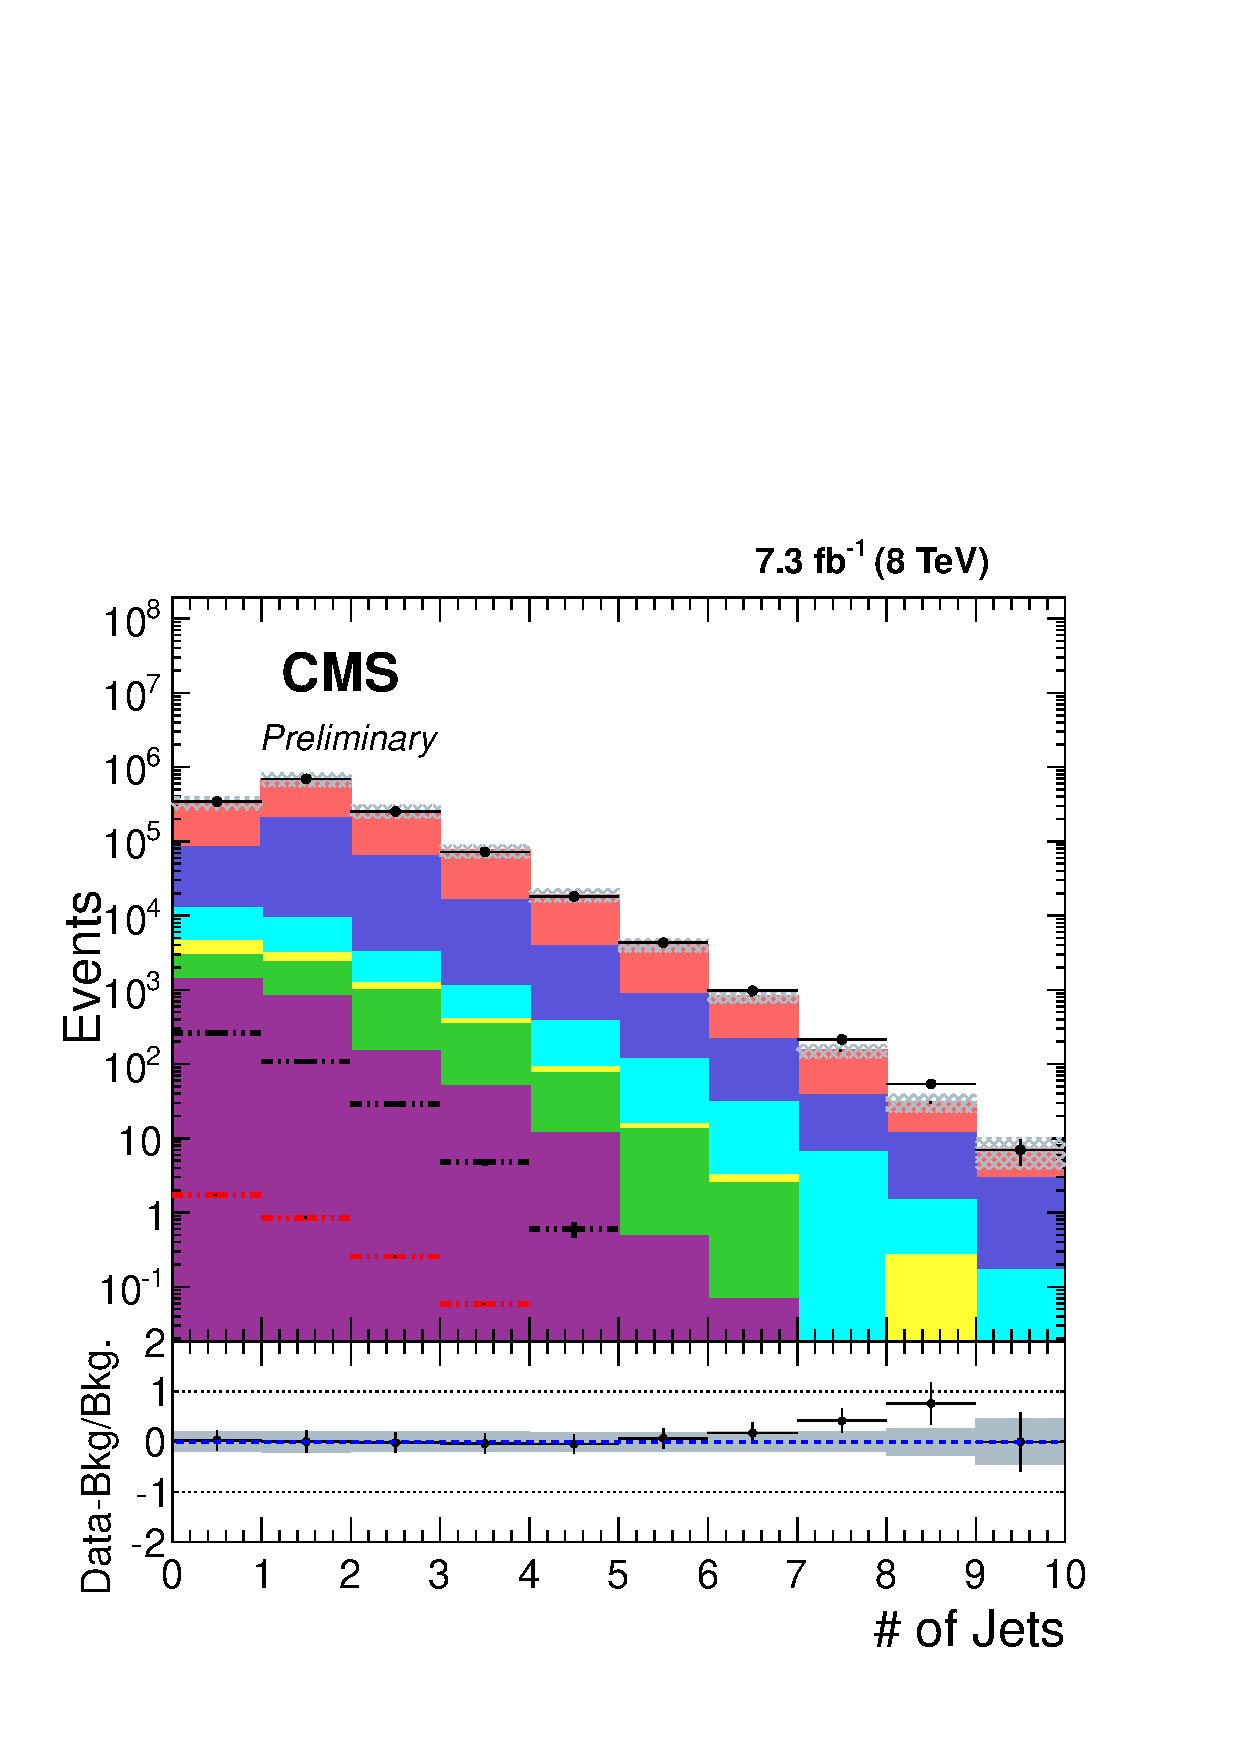
\includegraphics[width=8.3cm,height=8.3cm]{analysis_figs/final_njets.pdf}}
  {\label{fig:HT}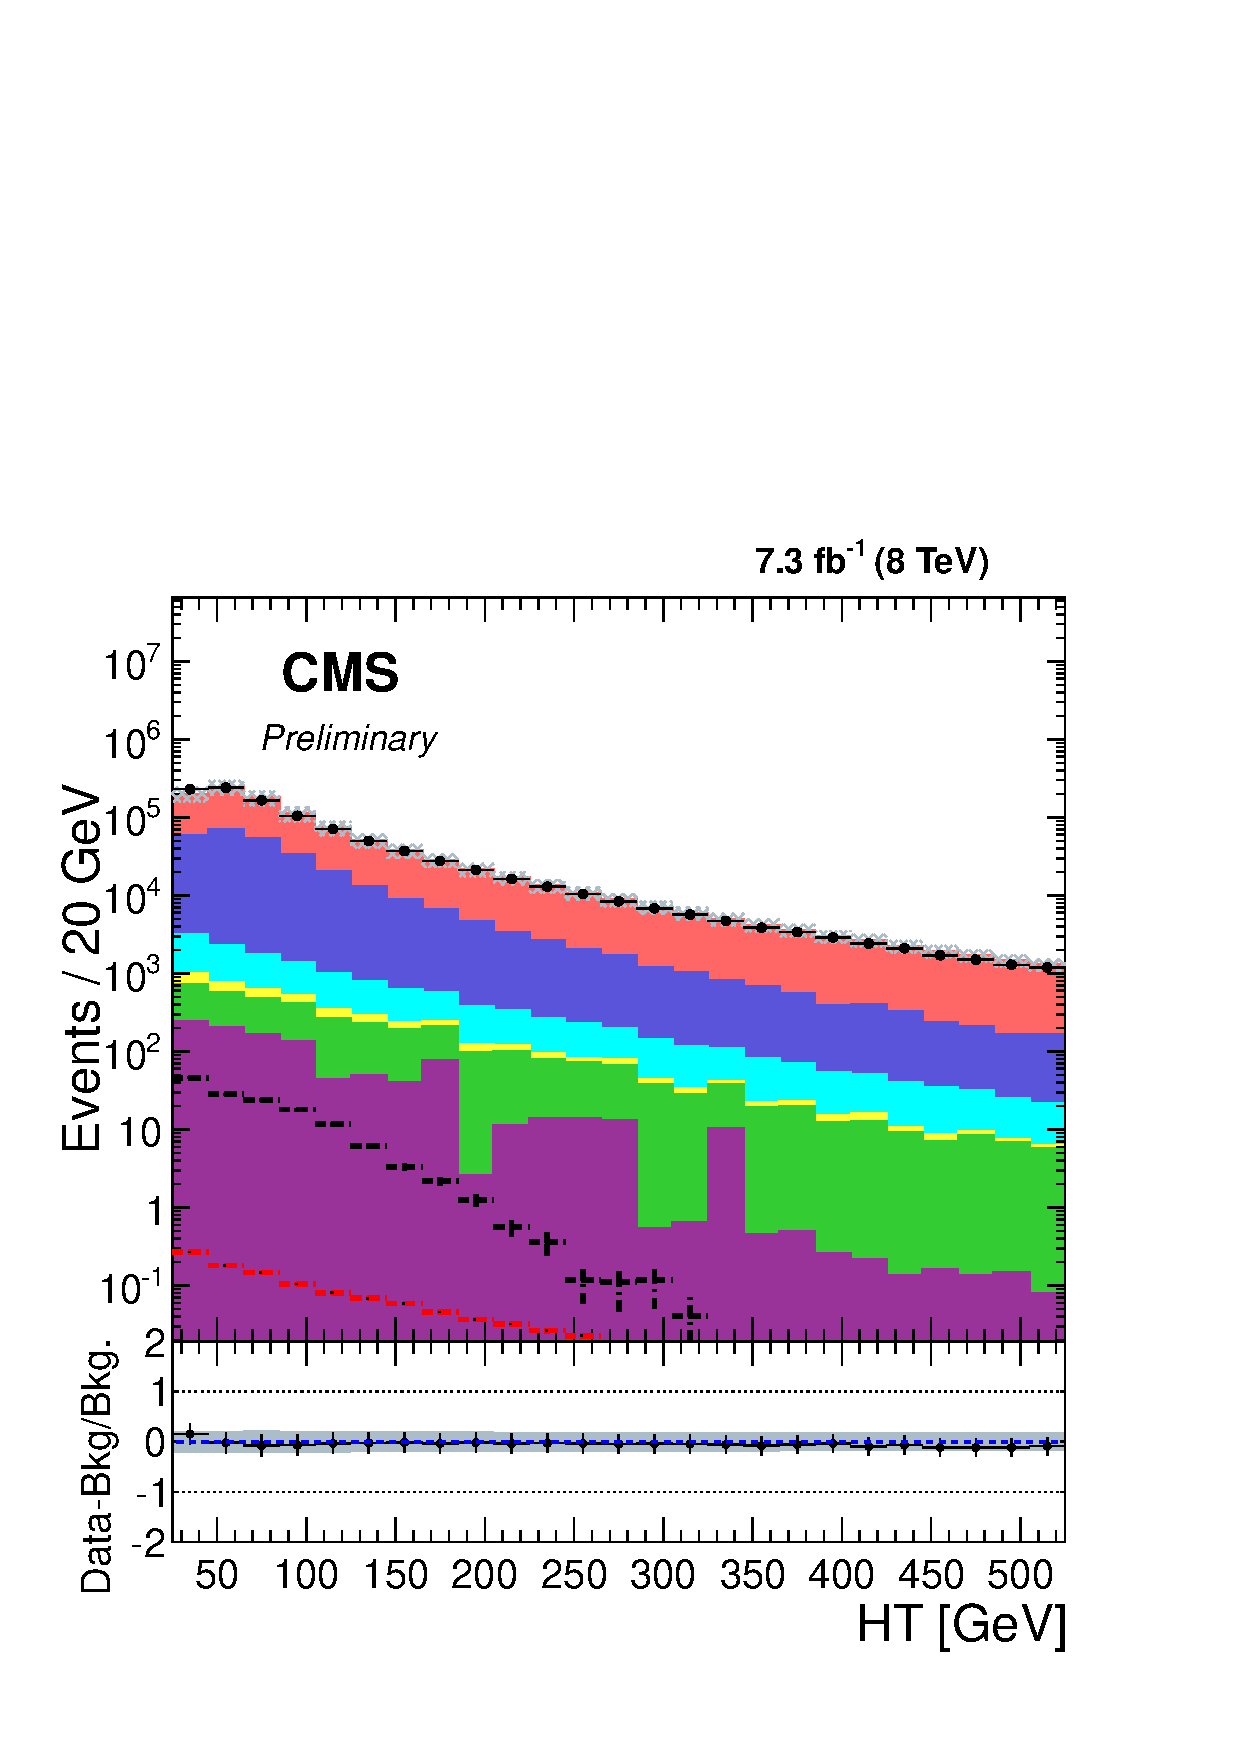
\includegraphics[width=8.3cm,height=8.3cm]{analysis_figs/final_HT.pdf}}
 \caption{Number of Jet (left) and HT (right) distributions in the Photon + Jet control Region. }
 \label{fig:control_jet}
\end{figure}


\subsection{Lepton Control Region}

We also studied the region dominated by the $W\gamma$ process. For the Lepton Control Region phase space, we select events based on the preselection but with a loose muon or an electron (inverting the lepton veto). Due to the lepton requirement, in this very minimal signal contamination is observed. Table~\ref{tab:WG_CRI} summarizes the yields obtained for the lepton control region. Fig.~\ref{fig:WG_CRI} shows the data vs background prediction for the photon \pt and the \met in the control region. Data and expectations agree within errors.

\begin{table}[!hp]
\center
{
\begin{tabular}{|c|c|}
\hline
Process & Estimate \\
\hline
$\gamma +$ jets                          & 1994 $\pm$ 319 \\
${\rm jet}\rightarrow \gamma$            & 1591 $\pm$ 557 \\
${\rm e} \rightarrow \gamma$             & 765 $\pm$ 45  \\
$W(\to \ell\nu)+\gamma $                 & 2636 $\pm$ 131 \\
$Z( \to l \bar{l} )+\gamma    $          & 267 $\pm$ 16 \\
Other                                    & 1696 $\pm$ 83 \\
\hline
Total background                         & 8953 $\pm$ 1279 \\
\hline
Data                                     & 8247  \\
\hline
\end{tabular}
\caption{Expected yields after the lepton control region selections.}
\label{tab:WG_CRI}
}
\end{table}


\begin{figure}[!hp]
\centering
{\label{fig:leptonPt}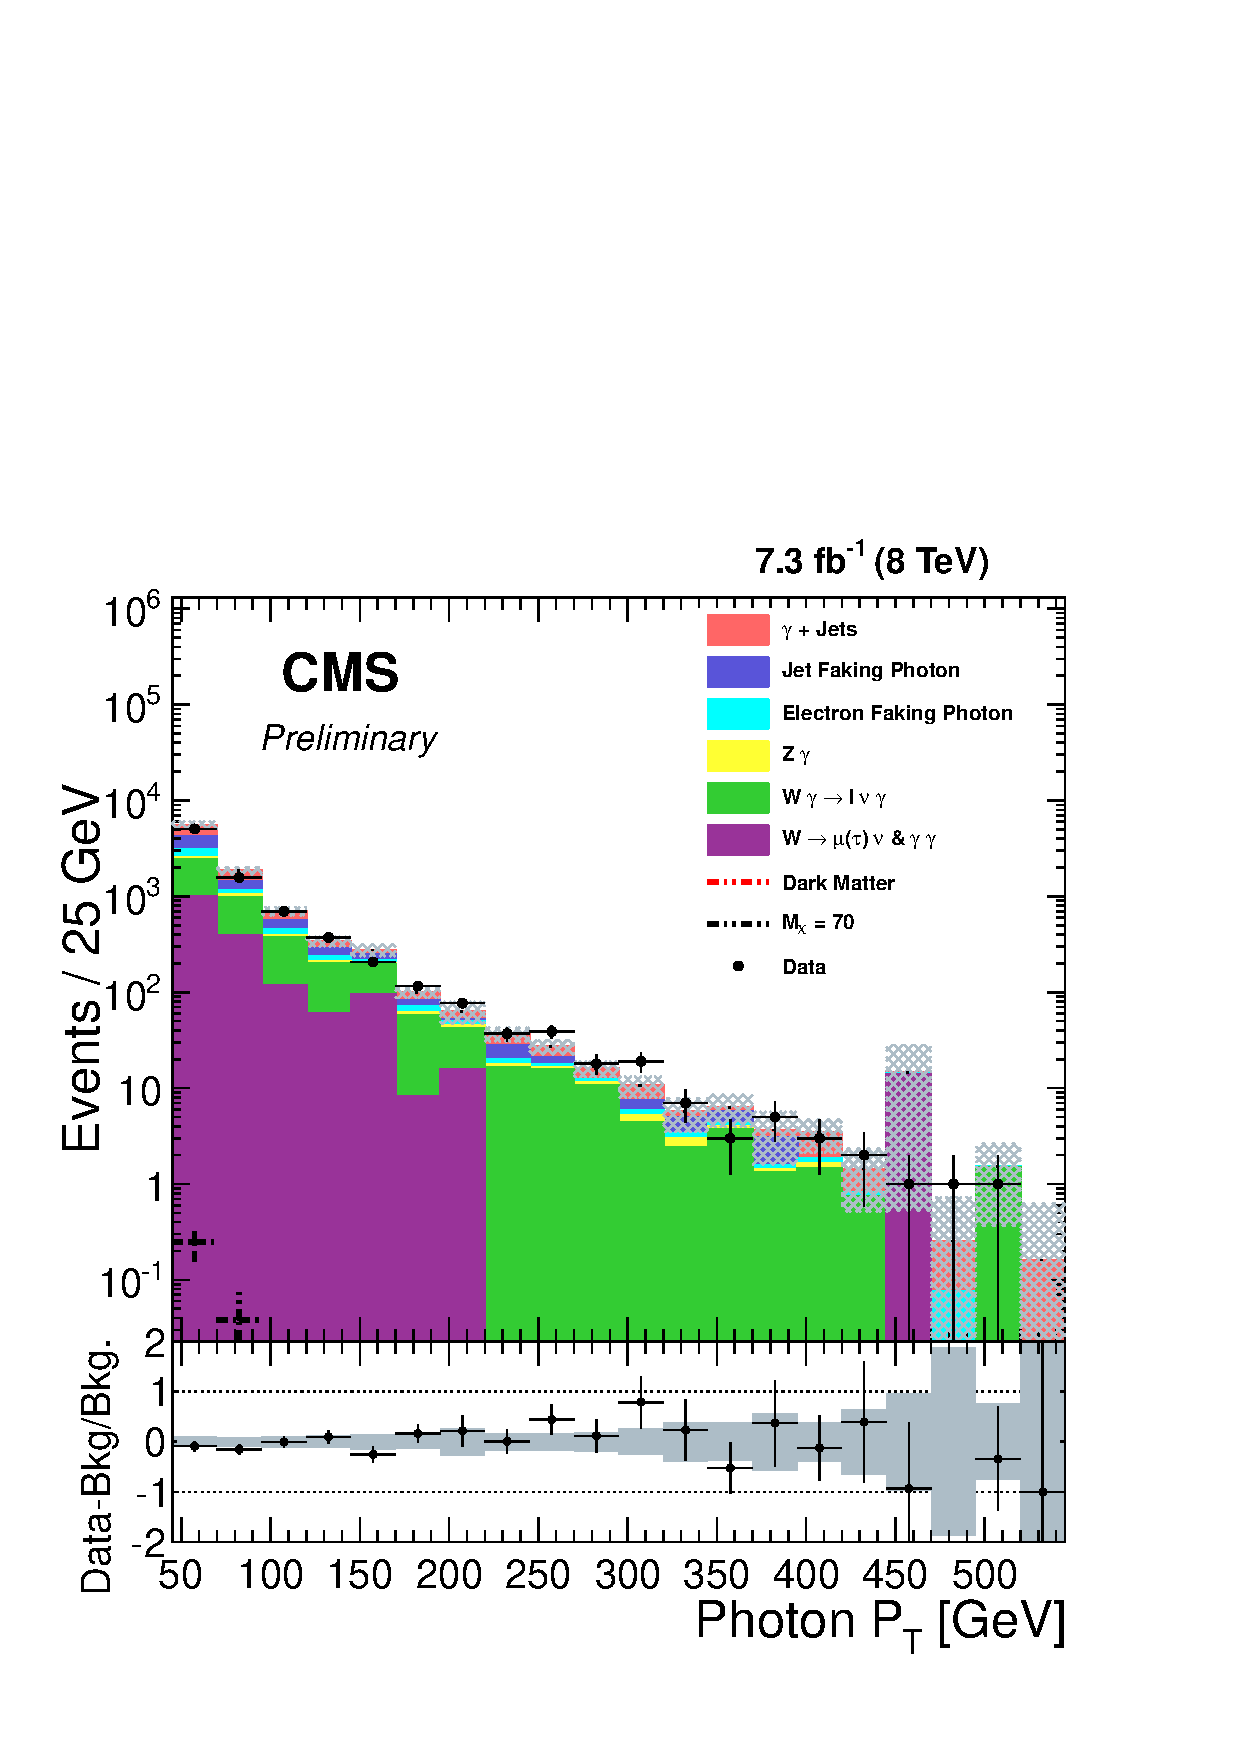
\includegraphics[scale=0.4]{analysis_figs/lepton_pt.pdf}}
{\label{fig:leptonMET}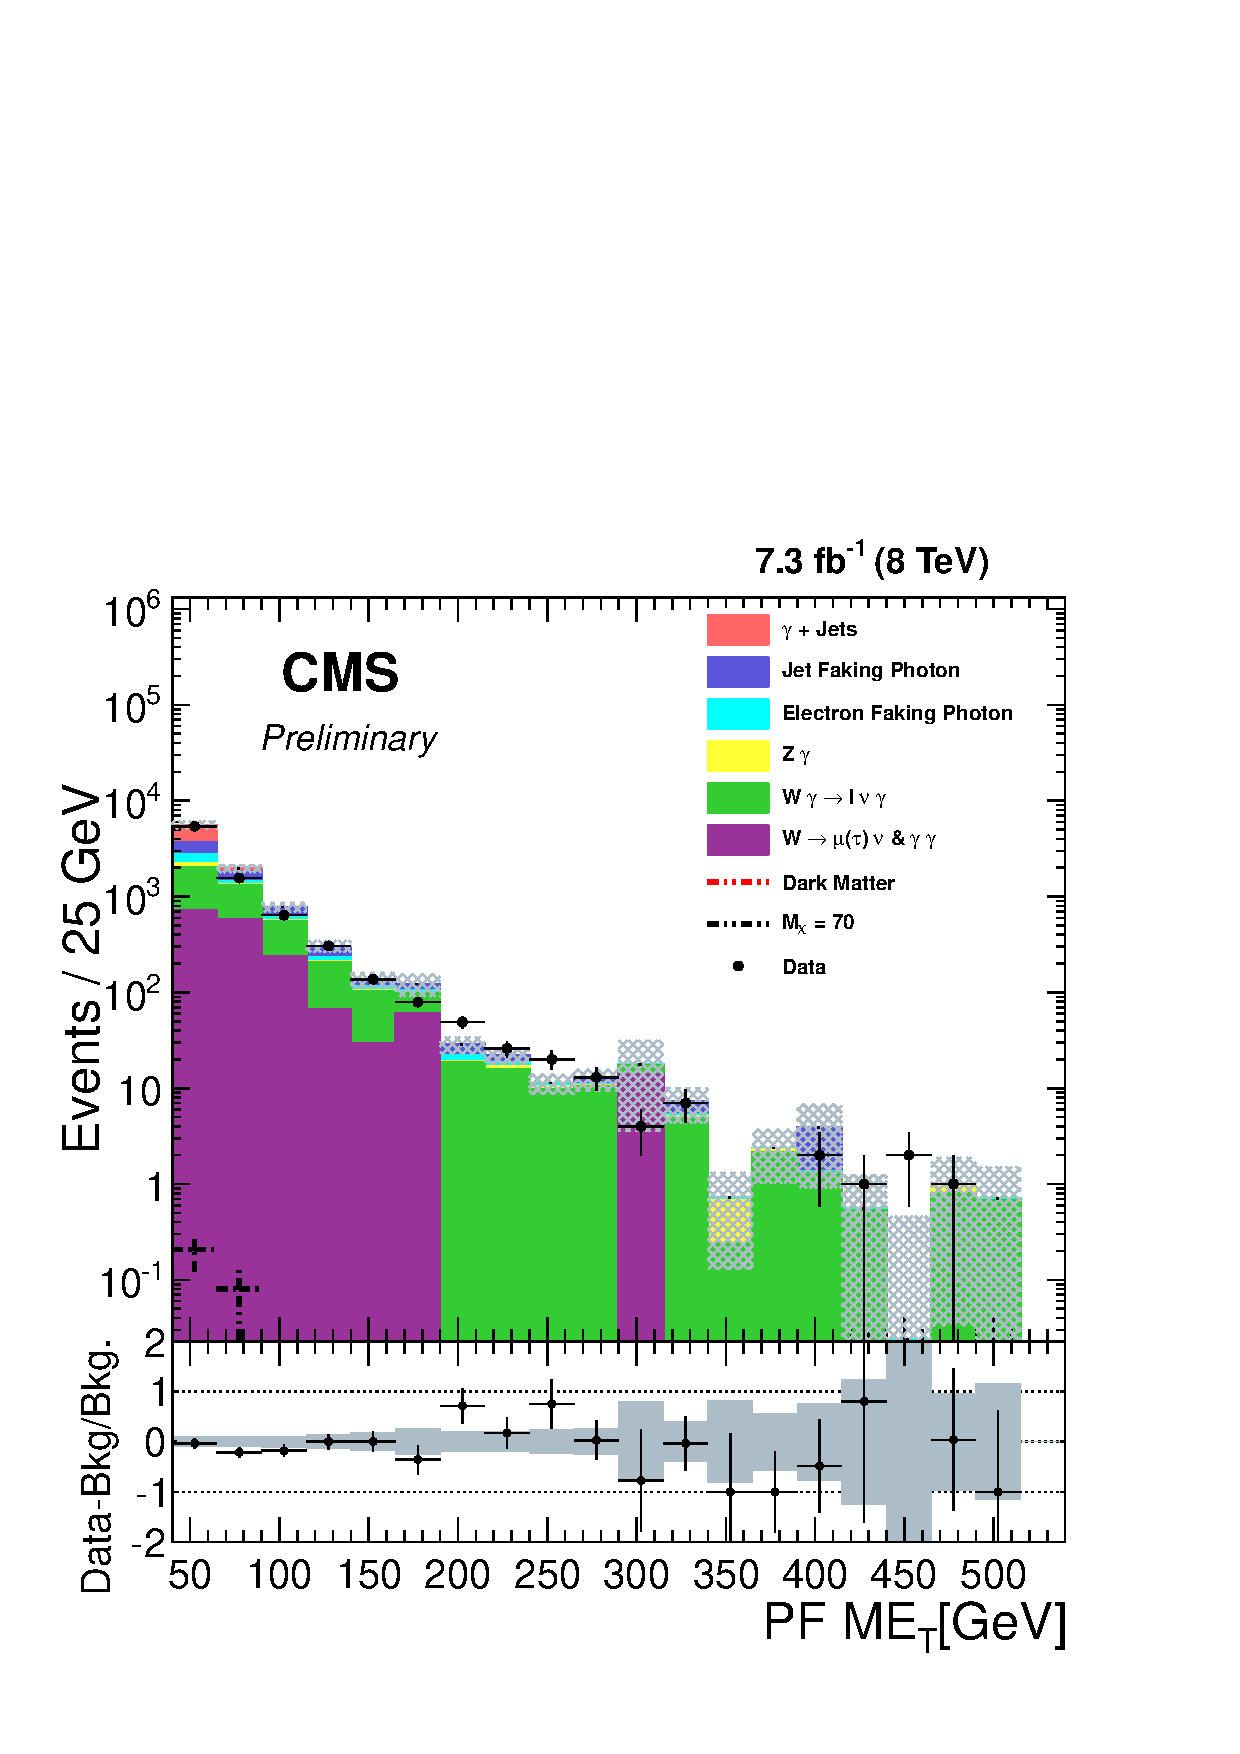
\includegraphics[scale=0.4]{analysis_figs/lepton_met.pdf}}
\caption{ Data vs background prediction comparison for the photon \pt and the \met in the lepton control region.}
\label{fig:WG_CRI}
\end{figure}

